% This must be in the first 5 lines to tell arXiv to use pdfLaTeX, which is strongly recommended.
\pdfoutput=1
% In particular, the hyperref package requires pdfLaTeX in order to break URLs across lines.

\documentclass[11pt]{article}

\usepackage{hyperref}
\usepackage{listings}
\usepackage{xcolor}

\definecolor{codegreen}{rgb}{0,0.6,0}
\definecolor{codegray}{rgb}{0.5,0.5,0.5}
\definecolor{codepurple}{rgb}{0.58,0,0.82}
\definecolor{backcolour}{rgb}{0.95,0.95,0.92}

\lstdefinestyle{mystyle}{
    backgroundcolor=\color{backcolour},   
    commentstyle=\color{codegreen},
    keywordstyle=\color{magenta},
    numberstyle=\tiny\color{codegray},
    stringstyle=\color{codepurple},
    basicstyle=\ttfamily\footnotesize,
    breakatwhitespace=false,         
    breaklines=true,                 
    captionpos=b,                    
    keepspaces=true,                 
    numbers=left,                    
    numbersep=5pt,                  
    showspaces=false,                
    showstringspaces=false,
    showtabs=false,                  
    tabsize=2
}

\lstset{language=Python,
	style=mystyle}

% Change "review" to "final" to generate the final (sometimes called camera-ready) version.
% Change to "preprint" to generate a non-anonymous version with page numbers.
\usepackage[final]{acl}

% Standard package includes
\usepackage{times}
\usepackage{latexsym}

% For proper rendering and hyphenation of words containing Latin characters (including in bib files)
\usepackage[T1]{fontenc}
% For Vietnamese characters
% \usepackage[T5]{fontenc}
% See https://www.latex-project.org/help/documentation/encguide.pdf for other character sets

% This assumes your files are encoded as UTF8
\usepackage[utf8]{inputenc}

% This is not strictly necessary, and may be commented out,
% but it will improve the layout of the manuscript,
% and will typically save some space.
\usepackage{microtype}

% This is also not strictly necessary, and may be commented out.
% However, it will improve the aesthetics of text in
% the typewriter font.
\usepackage{inconsolata}

%Including images in your LaTeX document requires adding
%additional package(s)
\usepackage{graphicx}

% If the title and author information does not fit in the area allocated, uncomment the following
%
%\setlength\titlebox{<dim>}
%
% and set <dim> to something 5cm or larger.

\title{How Can Linguistic Features Be Used for Modern and Classical Chinese Identification?}

\author{Author \\
  Student ID: 36506921 \\}

\begin{document}
\maketitle
\section{Introduction}

Natural language processing plays an important role in various fields, especially in artificial intelligence. However, I found that the development of AI in China is relatively slow, especially for practical models like CHAT GPT, which can be used directly by non-professionals for free with high accuracy, and baidu-unit, which is the most commonly used LLM in China; however, its performance is not very good, e.g., in the aspect of security, the protection of personal information of baidu-unit is relatively weak. 

What is the reason for the slow development of LLM in China? Perhaps it is due to the difference in language families. English belongs to the Indo-European language family, while Chinese belongs to the Sino-Tibetan language family. There are correspondences and similarities between certain phonological, lexical and grammatical rules between the same language families. Therefore, since the early development of computer science and programming languages took place mainly in countries where English is the native language, this may give English an inherent advantage in areas such as natural language processing. And due to the difference in the length of development, the Chinese corpus also has the disadvantage of the size and richness of the dataset. Therefore, in this research I will use natural language processing algorithms to study Chinese language. I will compare the results based on different linguistic features extraction for the distinction between modern Chinese and classical Chinese.

The biggest difference between modern Chinese and classical Chinese is the difference in grammar. The grammar of the classical Chinese language is more streamlined, and there are many words or phrases with completely different meanings from the modern Chinese language, and there is also a big difference in the participle structure, but there is no difference between the two in the use of words and phrases, so it will be a little bit difficult to differentiate between these two languages. In this paper, we will compare the two languages through different feature extraction to study which feature is more suitable for the distinction and discuss the reasons.

\section{Related Work}

The first difficulty in this research is the collection of the corpus. This is because Chinese corpus resources are relatively few and none of them are open source. Fortunately I found a chatbot project on GitHub, which provides open source Chinese corpus. Similarly, in other projects I acquired corpora of classical Chinese. For pre-processing, I only retained Chinese characters and punctuation marks in the corpus for the purpose of word and sentence division. Then I choose TF-IDF, ngram and BoW for feature extraction, the advantages of these method I will explain in later chapters. Finally I choose to use Random Forest model for classification. I tried SVM before this, but the results were not satisfactory. Ultimately I analyse the performance of these feature extraction methods compared to each other and discuss the reasons for this.

\section{Data}

Firstly, in terms of corpus selection I chose to get it from the most commonly used app, which is Weibo. This app is similar to X (also known as twitter), on which most Chinese people share their daily life, so this part of the corpus is very close to daily life. On the contrary, for the corpus selection of classical Chinese, I chose a variety of ancient books. This is because classical Chinese is a written language in itself, and even in ancient times, people did not choose to use classical Chinese exclusively when they spoke. The total size of the modern Chinese and classical Chinese corpus is about 1GB, and after word segmentation, it is about 500 million words.

In addition, in the preprocessing of the data, the minimum granularity I chose was sentences. This is because modern Chinese and classical Chinese have a large part of overlap in word usage, and the real difference between the two lies in the difference in grammar and the different meanings of certain same words. Therefore it is meaningless to classify them if we only rely on participle words. The two corpora are roughly equal in volume, and because of the high similarity in lexical usage, I assigned a greater proportion to the training set in order to be able to make the model more accurate during training. And I did not remove stop words during preprocessing. Although these uncommon or meaningless words cannot provide effective help in the field of semantic analysis, these stop words are very useful in the classification task of two languages with similar grammar but different word usage. And it can also be seen from the statistics of word segmentation results that both languages have a large proportion of particles, but the content of the particles is completely different. This can help the algorithm distinguish the two well.

\section{Methodology}

In this research I used a comparison of results from different means of feature extraction to verify the strengths and weaknesses of these methods and to derive the impact of these methods on language classification.

Specifically, in the preprocessing stage, I used different word segmentation algorithms for two different corpora to cope with different grammatical structures. For modern Chinese, I used the jieba word segmentation algorithm for word segmentation. For classical Chinese, I use the thulac algorithm introduced by Tsinghua University for word segmentation. Since I reserved commonly used Chinese punctuation marks in the preprocessing stage, this allowed me to perform sentence segmentation before feature extraction.

The focus of this study is on the feature extraction stage. I chose three feature extraction methods, namely N-gram (unigram and bigram together), TF-IDF and Bag-of-Words model. Each of these three models has its own advantages and disadvantages. The N-gram model is a statistical language model used to predict the probability of the $N$th word based on the first $N-1$ words. It estimates these probabilities by calculating the frequency of occurrences of observed word sequences\cite{goodman2001bit}. Since the N-gram model is very dependent on context, which is similar to the grammatical structure of language, and both modern Chinese and classical Chinese follow grammatical rules, N-gram can be well used to extract features. TF-IDF is an effective weight calculation method that can distinguish keywords and common words in documents and enhance the relevance of search results. However, TF-IDF only considers the frequency of words and does not consider the position of the word in the document, the context, or the grammatical relationship between words\cite{brin1998anatomy}. Therefore, it is inferior to N-gram in this aspect. The bag-of-words model is a simple method for processing text data. Its basic idea is to treat text as a collection of words without considering the order and grammatical relationship between words. In this model, each document is represented as a long vector, each dimension of this vector corresponds to a word in the vocabulary, and the value of each dimension reflects the frequency of that word in the document\cite{manning2008introduction}. However, analysis based solely on frequency will ignore synonyms, which is also a shortcoming of the bag-of-words model.

Finally, I use the SGD model for training and prediction. Since my data volume is about 1G, with about 500 million words, even though I use sentence segmentation, there are still tens of millions of data that need to be analyzed. Therefore, the more general SVM model is not suitable for my large amount of data. My SVM model took several hours to complete but the SGD model could be trained in a few minutes. When the amount of data is large, it is obvious that SGD is more suitable.


\section{Results and Findings}

The performance of these three models is similar. In some cases, they perform well, but in some cases they perform very poorly. The specific performance is that they all show low precision($p$) and high recall rate($r$) in the prediction of classical Chinese, while the prediction of modern Chinese is exactly the opposite. These formulas are as follows.

\begin{equation}
  \label{eq:example}
  p = \frac{TP}{TP+FP}
\end{equation}

\begin{equation}
  \label{eq:example}
  r = \frac{TP}{TP+FN}
\end{equation}

\begin{equation}
  \label{eq:example}
  F1 = 2 \times \frac{precision\times recall}{precision+recall}
\end{equation}

According to the calculation formulas of precision and recall, it can be seen that a lot of modern Chinese is misclassified as classical Chinese. This is an error trend, and it is this trend that shows different precision and recall rates.

\begin{figure}[t]
  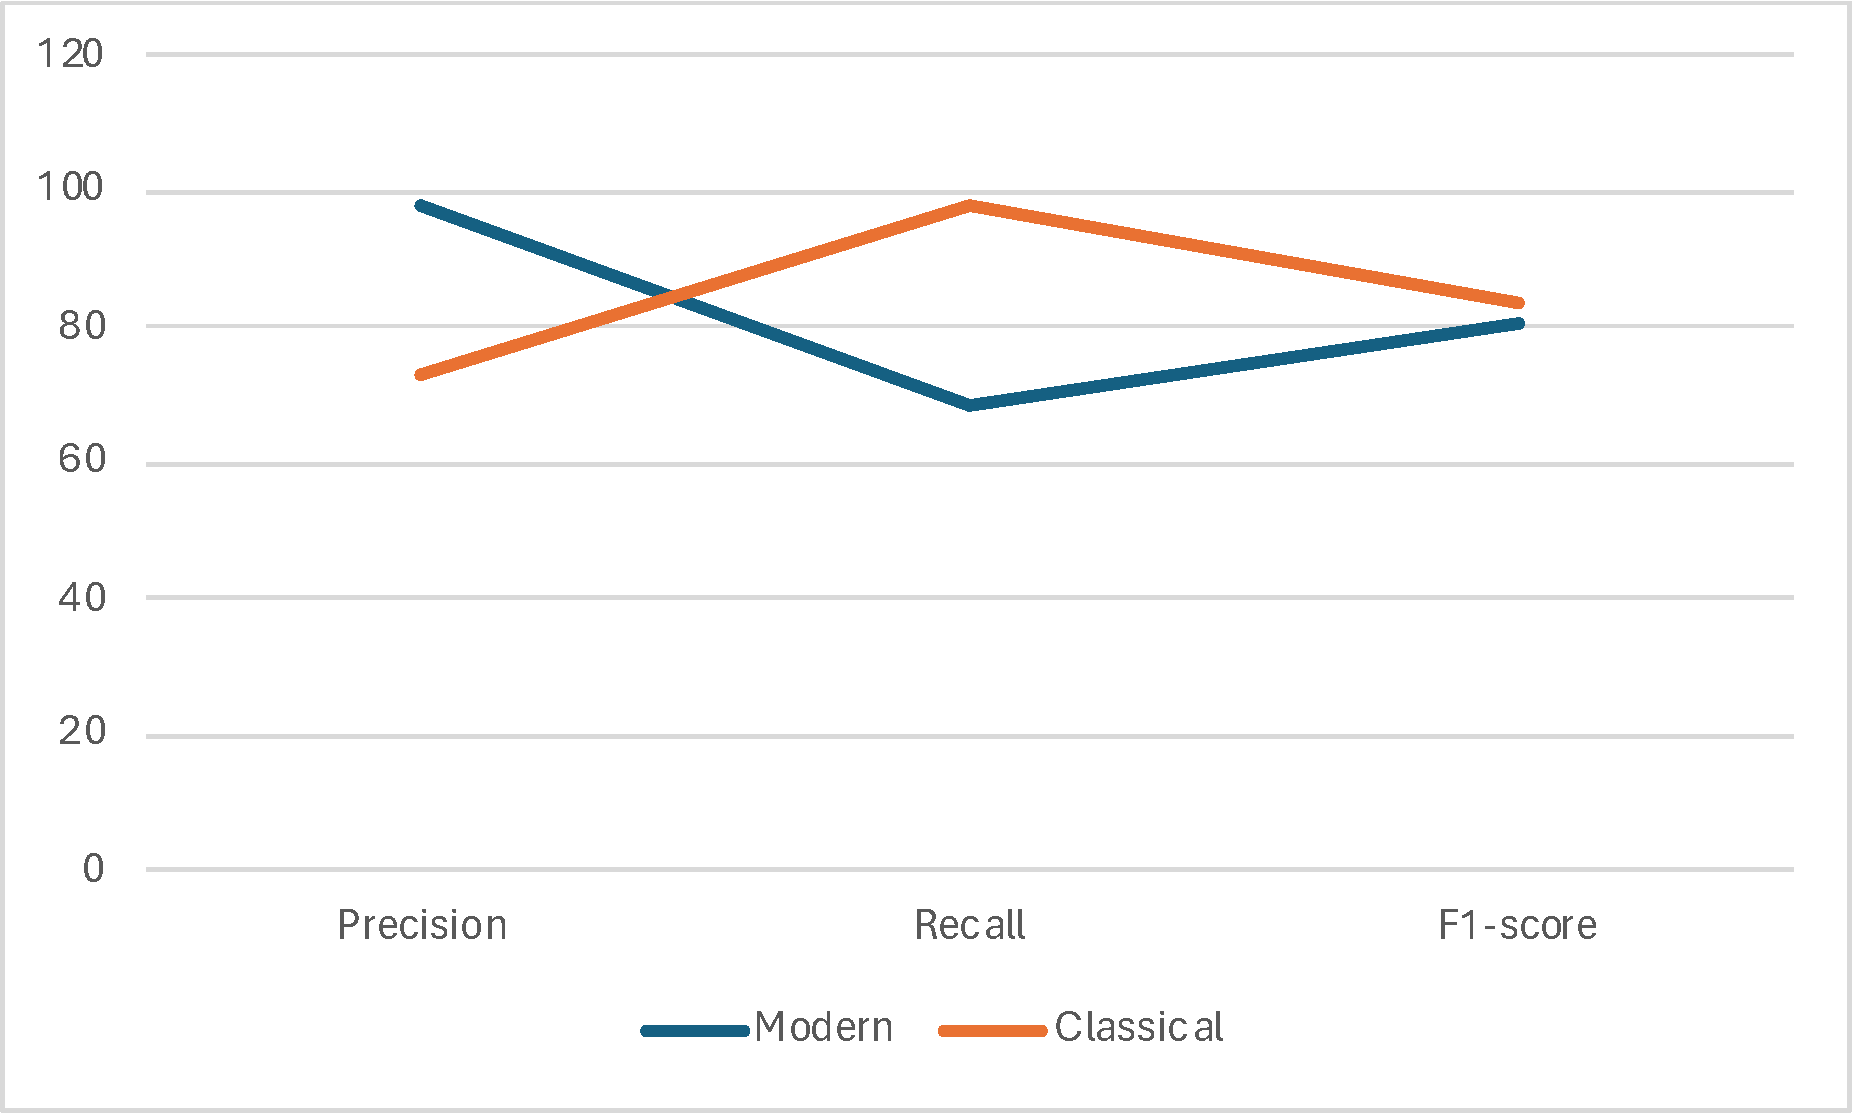
\includegraphics[width=\columnwidth]{figures/2.pdf}
  \caption{Average performance of the three models. Because the performance of the three models is very similar, taking the average here will not affect the accuracy of the analysis.}
  \label{fig:average}
\end{figure}

The language habits of modern Chinese and classical Chinese are indeed different. According to the word segmentation results, the words with the highest frequency are almost completely different, but the parts of speech are very similar. Therefore, although the semantics of the two are different, it can be seen that the grammar is relatively close. Therefore, it is inferred that the performance of N-gram should be relatively better. However, after verification, it was found that there was no obvious difference in the performance of these models in predicting classification. This may be a problem with the model parameter settings, or it may be a problem with the selection of the corpus. Because I did not choose the most official news data as the modern Chinese corpus, but chose Weibo data that is closer to life and spoken language, this may also lead to difficulties in distinguishing some commonly used terms.

\begin{figure}[t]
  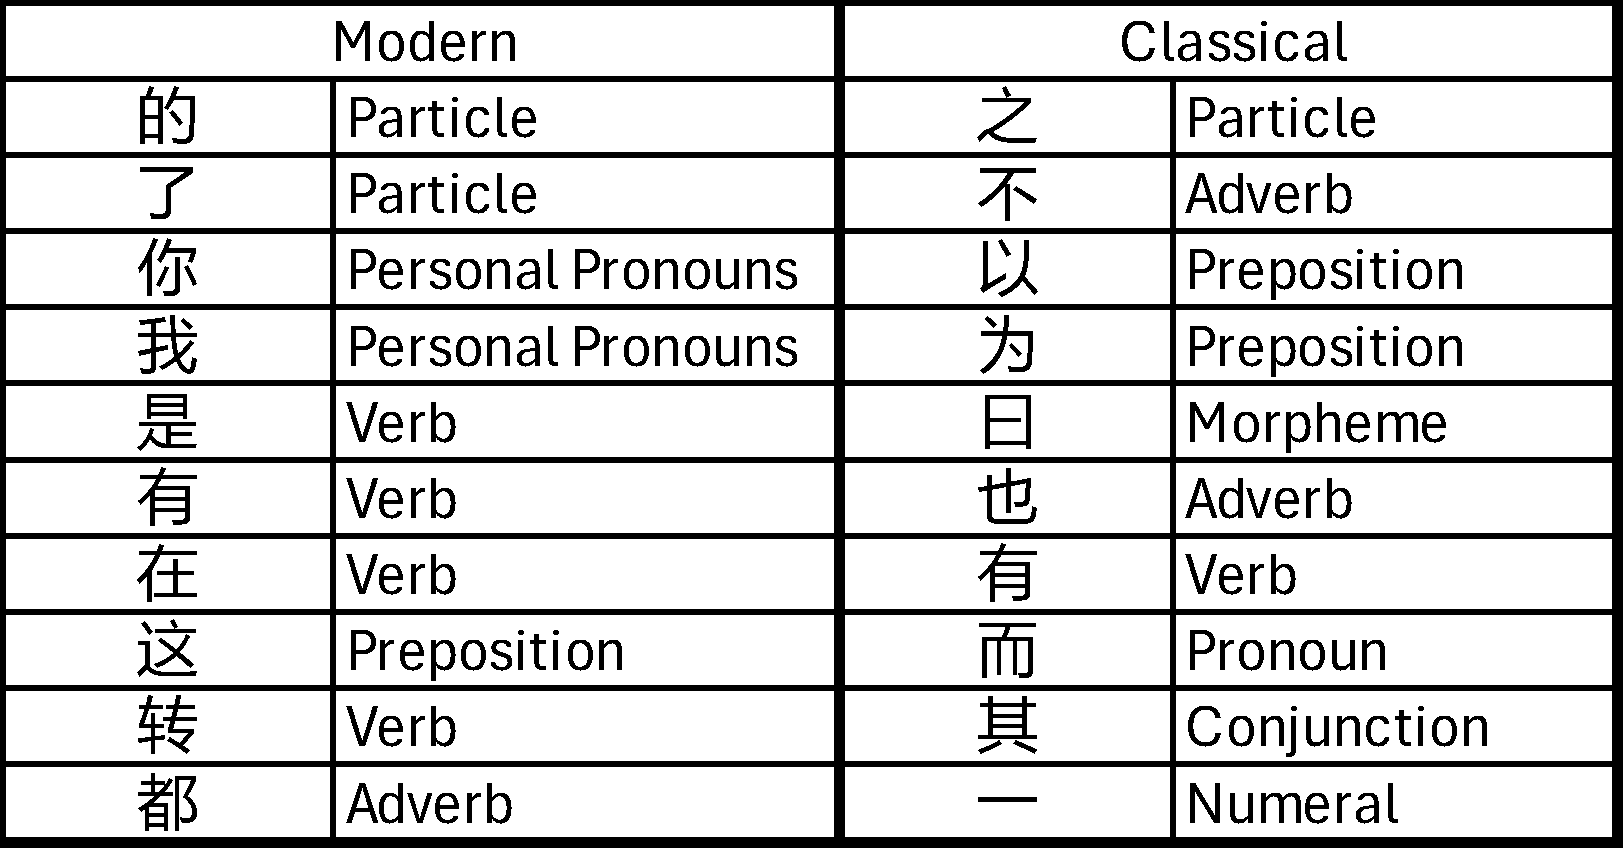
\includegraphics[width=\columnwidth]{figures/4.pdf}
  \caption{The predicted data performance of the other two models based on the N-gram model. Assume N-gram is 100.}
  \label{fig:language}
\end{figure}

However, see Figure \ref{fig:ngram}, taking the performance of N-gram in various situations as 100 as a benchmark, it can be seen that the performance of TF-IDF is the best, while the performance of the bag-of-words model is basically lower than or equal to N-gram . I think this gap is caused by differences in algorithm logic and grammatical differences in the languages in the corpus. First of all, neither TF-IDF nor the bag-of-words model considers context order, but TF-IDF reduces some of the words with the highest document frequency because these words may be meaningless connectives. It is this difference that leads to the best performance of the TF-IDF model and the worst performance of the bag-of-words model. It can also be seen from Figure \ref{fig:language} that among the 10 words with the highest frequency in the corpus after word segmentation, particles still account for the majority. My original consideration was that although particles cannot be used as effective units for semantic analysis, the differences in wording in language classification may be helpful for classification, so I did not remove these words. Obviously these words interfere with the classification of the algorithm. Subsequently, the stop words should be removed and the classification attempt should be made again.

\begin{figure}[t]
  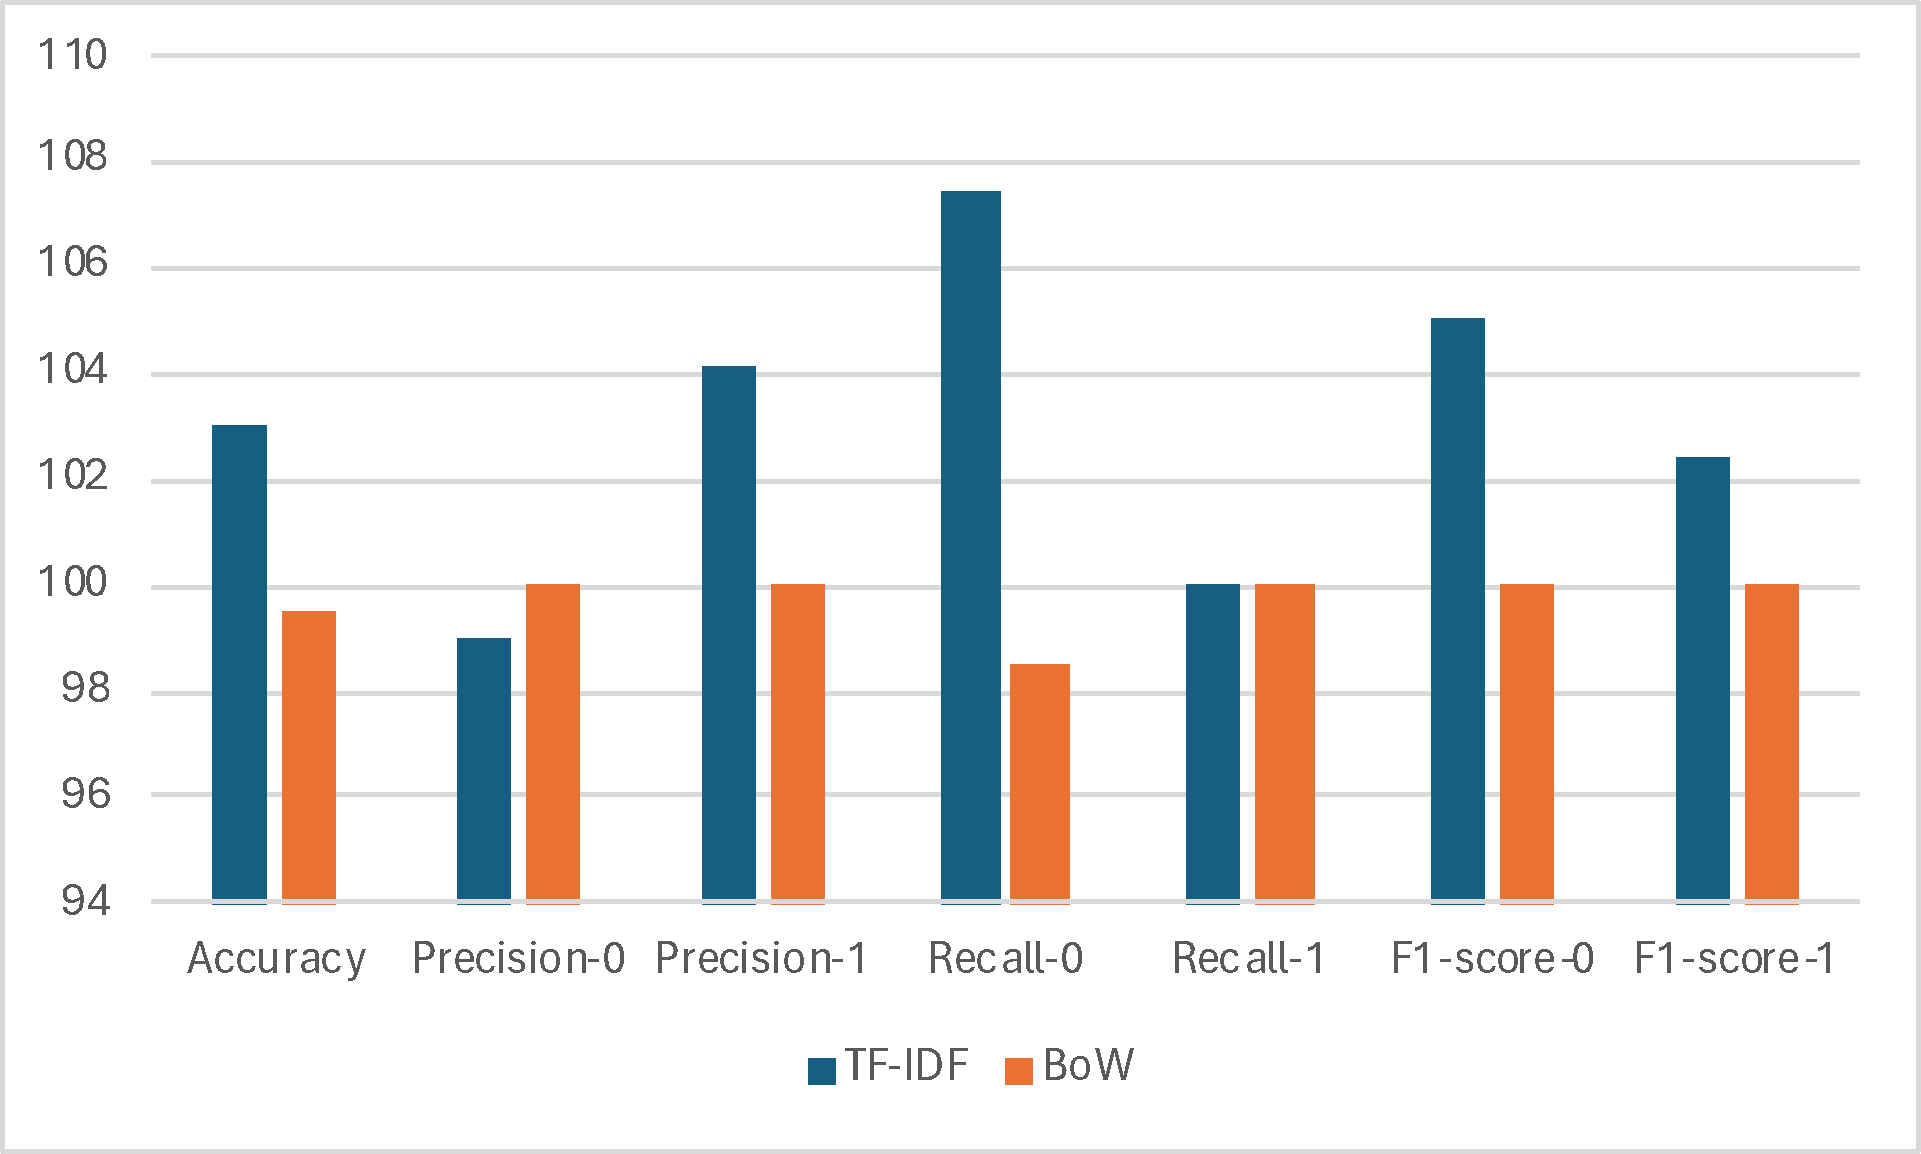
\includegraphics[width=\columnwidth]{figures/1.pdf}
  \caption{The predicted data performance of the other two models based on the N-gram model. Assume N-gram is 100.}
  \label{fig:ngram}
\end{figure}

It is worth noting that although the performance of the three is similar, their running time is different, see Table \ref{tab:time}. The performance of N-gram is good, but the running time is longer and the time efficiency is the lowest. The running time of other TF-IDF and bag-of-word models is basically the same, so when the amount of data is larger, the TF-IDF model should be used for modelling and prediction to ensure time efficiency. Of course, the actual performance of the bag-of-words model still needs to be compared after deleting stop words.

\begin{table}
  \centering
  \begin{tabular}{lc}
    \hline
    \textbf{Model} & \textbf{Running Time/s} \\
    \hline
    N-gram     & 22.72           \\
    TF-IDF     & 17.13           \\
    Bow     & 17.92          \\\hline
  \end{tabular}
  \caption{The running time of these three models.}
  \label{tab:time}
 \end{table}

\section{Conclusions and Future Work}

In summary, N-gram, TF-IDF and bag-of-words models have differences in time efficiency, but there is not much difference in overall classification results. Therefore, the preliminary conclusion is that if there are no high requirements for prediction accuracy, then it is recommended to use the TF-IDF model or the bag-of-words model. The time efficiency of the two is the best, and the former is also the best in terms of prediction accuracy. Although the difference is not huge.

In the future, it is still necessary to remove stop words from the data and delete particles or personal pronouns such as you, me and him to ensure that the logic of the bag-of-words model and TF-IDF model can be better used. Other feature extraction methods will also be tried, because it is obvious that even though N-gram takes into account the connection between contexts, this does not bring advantages. Therefore, it is likely that the focus of Chinese classification tasks in different periods will be on word frequency. This is not consistent with my original idea, because I think the grammar of classical Chinese and modern Chinese should be different. This may be because the difference between the two is mainly reflected in the difference in wording rather than grammar. The actual difference in grammar is much smaller than the difference in wording, so the advantages of N-grams are not reflected. We will consider using word frequency for more analysis in the future.

\section*{Acknowledgments}

The corpus comes from:

\href{https://github.com/codemayq/chinese-chatbot-corpus}{Modern Chinese Corpus}

\href{https://github.com/NiuTrans/Classical-Modern}{Classical Chinese Corpus}

The segmentation libraries:

Modern Chinese: \href{https://github.com/fxsjy/jieba}{jieba}

Classical Chinese: \href{http://thulac.thunlp.org/}{thulac}

\bibliography{custom}

\onecolumn
\appendix

\section{Pre-processing}
\label{sec:appendix}

\lstinputlisting[language=Python]{./codes/preprocessing.py}
\clearpage

\section{Modelling}
\label{sec:appendix}
\lstinputlisting[language=Python]{./codes/model.py}



\end{document}